\section{Automaten}

\begin{frame}{Endliche Automaten}
	Ein deterministischer endlicher Automat...
	\begin{itemize}
		\item besteht aus endlich vielen Zuständen
		\item ist zu jedem Zeitpunkt in \emph{genau einem} dieser Zustände
		\item wechselt bei Eingabe \emph{genau eines} Zeichens den Zustand in \emph{genau einen, definierten} Folgezustand
		\item und gibt dabei ein Wort als Ausgabe aus
	\end{itemize}

	Die gültigen \enquote{Zustandswechsel} sind als Zustandsübergänge definiert.
\end{frame}

\begin{frame}{Anwendungen}
	\begin{itemize}
		\item Getränkeautomaten
		\item Textsuche
		\item Textersetzung
	\end{itemize}

	Für Beispiele zur Textsuche und Textersetzung: Übung~12, WS~15/16
\end{frame}

\mycomment{ % As a source for copy/pasting:
\begin{tikzpicture}[->,>=stealth,shorten >=1pt,auto,node distance=2.8cm,
semithick,initial text={}]
\tikzstyle{every state}=[fill=red,draw=none,text=white]

\node[initial,state] (A)                    {$q_a$};
\node[state]         (B) [above right of=A] {$q_b$};
\node[state]         (D) [below right of=A] {$q_d$};
\node[state]         (C) [below right of=B] {$q_c$};
\node[state]         (E) [below of=D]       {$q_e$};

\path (A) edge              node {0,1,L} (B)
		  edge              node {1,1,R} (C)
(B) edge [loop above] node {1,1,L} (B)
	edge              node {0,1,L} (C)
(C) edge              node {0,1,L} (D)
	edge [bend left]  node {1,0,R} (E)
(D) edge [loop below] node {1,1,R} (D)
	edge              node {0,1,R} (A)
(E) edge [bend left]  node {1,0,R} (A);
\end{tikzpicture}	
}

\subsection{Mealy-Automaten}
\begin{frame}{Ein einfacher Automat}
	\begin{center}
		\begin{tikzpicture}[->,>=stealth,shorten >=1pt,auto,node distance=2.8cm,
			semithick,initial text={}]
			\tikzstyle{every state}=[]
			
			\node[initial,state] (A)                    {$a$};
			\node[state]         (M) [right of=A] 	    {$m$};
			
			\path (A) edge [loop above] node {\word 1|\word 0} (A)
			          edge [loop below]  node {\word 0|\word 1} (A)
			          edge 					  node {\word{2}|\word{X}} (M)
			      (M) edge [loop right] node {$\stackedtight{\word 0|\word X \\ \word 1|\word X \\ \word 2|\word X}$} (M);
			      %(M) edge [loop right] node {\word 1|\word X} (M)
			      %(M) edge [loop below] node {\word 2|\word X} (M);
		\end{tikzpicture}
	\end{center}
	\pause
	Eingabe: \word{011101} \?> Ausgabe: \word{100010} \\
	Eingabe: \word{011102} \?> Ausgabe: \word{10001X} \\
	Eingabe: \word{012101} \?> Ausgabe: \word{10XXXX} \\ \pause
	\smallskip
	\impl Der Automat negiert das Eingabewort bitweise. \\
	(Frisst er ne \word 2, so isser beleidigt. \smiley)
\end{frame}

\begin{frame}{Mealy-Automat}
	Bei einem Mealy-Automaten findet die Ausgabe \textbf{bei den Zustandsübergängen} statt.
	\begin{Definition}
		Ein \textbf{Mealy-Automat} $ A = (Z,z_0,X,f,Y,g)$ besteht aus...
		\begin{itemize}
			\item einer endlichen Zustandsmenge $Z$ 
			\item einem Startzustand $z_0$
			\item einem Eingabealphabet $X$ 
			\item einer Zustandsübergangsfunktion $f \from Z\times X \functionto Z $
			\item einem Ausgabealphabet $Y$
			\item einer Ausgabefunktion $g \from Z\times X \functionto Y^* $ 
		\end{itemize}						
	\end{Definition}
\end{frame}

\begin{frame}{}
	\begin{block}{Graphische Darstellung}
		\begin{itemize}
			\item Oft malt man Automaten hin. (Achtung: Die formale Schreibweise wird trotzdem auch im Studium verwendet! Also auswendig lernen!)
			\item Zustände sind \textbf{Knoten} und Übergänge sind \textbf{gerichtete Kanten} in einem Graphen. \\
			Kanten\textbf{beschriftung}: „$\langle\text{Eingabe}\rangle | \langle\text{Ausgabe}\rangle$“
			\item \textbf{Der Startzustand wird mit einem Pfeil \enquote{aus dem Nichts} gekennzeichnet!}  \pause
			\implitem \textbf{NICHT VERGESSEN!} Kostet sonst Punkte! \textbf{Immer!}
		\end{itemize}
		
	\end{block}
\end{frame}

\begin{frame}{Beispiel: Automatengraphen}
	%\vspace{-1\baselineskip} 
	%\hspace{-\baselineskip}
	
\includegraphics[page=3,trim=18px 47px 18px 14px,clip]{U12.pdf}	
\end{frame}

%% Übung: Beispiel
%\setbeamercolor{background canvas}{bg=}


\begin{frame}{Eingabe eines Zeichens}
	Was ist die Zustandsübergangsfunktion $f$? \\ \pause
	\medskip
	Haben
	\begin{itemize}
		\item aktuellen Zustand $z \in Z$
		\item eingelesenes Zeichen $x \in X$
	\end{itemize}
	\impl $f$ liefert den Folgezustand $z_\text{neu}$, in welchem der Automat danach ist.\\
	\medskip
	Formell: $$ f(z,x) = z_\text{neu} $$ 
\end{frame}

\begin{frame}{Eingabe eines Wortes}
	Was machen wir mit ganzen Wörtern? \\ \pause
	Wir definieren uns ganz analog
	\begin{block}{Zustandsübergangsfunktion extended}
	\begin{align*}
		 	f_*(z,\eps) &:= z \\
		 	\forall w\in X^* , \, x\in X : \quad  f_*(z,wx) &:= f\left(f_*(z,w),x\right) 
	\end{align*}
	\end{block}
	\pause Was macht diese Funktion? \\ \pause
	\medskip
	Haben
	\begin{itemize}
		\item aktuellen Zustand $z \in Z$
		\item eingelesenes Wort $w \in X^*$
	\end{itemize}
	\impl $f_*$ liefert den \textbf{Endzustand} $z_\text{ende}$, in welchem der Automat \textbf{nach dem Wort} dann ist.
	Formell: $$ f_*(z,w) = z_\text{ende} $$
	%Bei Eingabe eines Wortes $w$ und Anfangszustand $z$ gibt sie den Zustand $z' = f_*(z,w)$ aus, in dem der Automat enden wird. 
\end{frame}
	
\begin{frame}{Eingabe eines Wortes}
	Definieren wir nun weiter 
	\begin{block}{Zustandsübergangsfunktion extended extended}
		\begin{align*}
			f_{**}(z, \eps) &:= z \\
			\forall w\in X^* , \, x\in X : \quad  f_{**}(z, xw)   &:= z \cdot f_{**}\!\left(f(z,x),w\right) \\
		\end{align*}
	\end{block}
	\pause Was macht diese Funktion? \\ \pause
	Diese Funktion gibt die Reihe aller \textbf{Zustände als Gesamtwort} aus, die der Automat bei Eingabe des Wortes $w$ im Startzustand $z$ durchläuft. Also: 
	$$ f_{**}(z, w) = z \* z_1 \* z_2 \cdots z_\text{ende} $$
\end{frame}

\begin{frame}{Eingabe eines Wortes}		
	Alternative Definition:
	\begin{block}{Zustandsübergangsfunktion extended extended}
		\begin{align*}
			f_{**}(z,\varepsilon) &= z \\
			\forall w \in X^* \ \forall x \in X : f_{**}(z,wx) &= f_{**}(z,w)\cdot f(f_*(z,w),x)	 
		\end{align*}
	\end{block}
\end{frame}

\begin{frame}{Beispiel $f, f_*, f_{**}$}
	\begin{center}
			\begin{tikzpicture}[->,>=stealth,shorten >=1pt,auto,node distance=2.8cm,
		semithick,initial text={}]
		\tikzstyle{every state}=[]
		
		\node[initial,state] (A)                    {$a$};
		\node[state]         (M) [right of=A] 	    {$m$};
		
		\path (A) edge [loop above] node {\word 1|\word 0} (A)
		edge [loop below]  node {\word 0|\word 1} (A)
		edge 					  node {\word{2}|\word{X}} (M)
		(M) edge [loop right] node {$\stackedtight{\word 0|\word X \\ \word 1|\word X \\ \word 2|\word X}$} (M);
		\end{tikzpicture}
	\end{center}
	\begin{align*}
		f(a, \word 2) &= m \\
		f(a, \word 0) &= a \\ 
	\end{align*}
	\pause  \vspace{-2.5\baselineskip}
	\begin{align*}
		f_*(a, \word{101}) &= \hphantom{aaa}a \\
		f_{**}(a, \word{101}) &= aaaa \\ 
	\end{align*}
	\pause  \vspace{-2.5\baselineskip}
	\begin{align*}
		f_*(a, \word{1021}) &= \hphantom{aaam}m \\
		f_{**}(a, \word{1021}) &= aaamm
	\end{align*}
\end{frame}

\begin{frame}{Ausgaben}
	Automaten können ja was ausgeben. \\
	\smallskip
	Erinnerung: Die Kanten sind beschriftet mit $x \mid y$ , wobei $x\in X$ und $y\in Y^* $. \\
	 \impl Für Eingabe $x$ wird das Wort $y$ ausgegeben. \\ 
	Formal: $$g(z,x) = y$$
\end{frame}

\begin{frame}{Ausgabefunktionen}
	\begin{block}{Ausgabefunktion extended}
		Wir können also analog zu $f_*$ und $f_{**}$ definieren
		\begin{threealign}
		\text{Für die letze Ausgabe: } \qquad g_* : Z\times X^* &\functionto& Y^* \\
		g_*(z,\varepsilon) &=& \varepsilon \\
		\forall w\in X^* \; \forall x\in X : g_*(z,wx) &=& g(f_*(z,w),x) \\ \\
		\text{Für das ganze Ausgabewort: } \qquad g_{**} : Z\times X^* &\functionto& Y^* \\ 
		g_{**}(z,\varepsilon) &=& \varepsilon \\
		\forall w\in X^* \; \forall x\in X : g_{**}(z,wx) &=& g_{**}(z,w)\cdot g_*(z,wx) 			
		\end{threealign} 
	\end{block}
	
	%\pause Dies gibt nun nicht die durchlaufenen Zustände bzw. den Abschlusszustand an, sondern die letzte Ausgabe bzw. alle durchlaufenen Ausgaben. 

\end{frame}

\begin{frame}{Beispiel $g, g_*, g_{**}$}
	\begin{center}
		\begin{tikzpicture}[->,>=stealth,shorten >=1pt,auto,node distance=2.8cm,
		semithick,initial text={}]
		\tikzstyle{every state}=[]
		
		\node[initial,state] (A)                    {$a$};
		\node[state]         (M) [right of=A] 	    {$m$};
		
		\path (A) edge [loop above] node {\word 1|\word 0} (A)
		edge [loop below]  node {\word 0|\word 1} (A)
		edge 					  node {\word{2}|\word{X}} (M)
		(M) edge [loop right] node {$\stackedtight{\word 0|\word X \\ \word 1|\word X \\ \word 2|\word X}$} (M);
		\end{tikzpicture}
	\end{center}
	\vspace{-\baselineskip}
	\begin{align*}
	g(a, \word 2) &= \word X \\
	g(a, \word 0) &= \word 1 \\ 
	\end{align*}
	\pause  \vspace{-2.5\baselineskip}
	\begin{align*}
	g_*(a, \word{101}) &= \hphantom{\word{01}}\word 0 \\
	g_{**}(a, \word{101}) &= \word{010} \\ 
	\end{align*}
	\pause  \vspace{-2.5\baselineskip}
	\begin{align*}
	g_*(a, \word{1021}) &= \hphantom{\word{01X}}\word X \\
	g_{**}(a, \word{1021}) &= \word{01XX} \\ 	\visible<+->{}
	\visible<+->{g_*(m, \word{0110}) &= }\visible<+->{\word X}
	\end{align*}
\end{frame}


\subsection{Moore-Automat}
\begin{frame}{Moore-Automat}
	Moore-Automaten sind fast genauso aufgebaut wie Mealy-Automaten.\\ \smallskip
	\textbf{Unterschied}: Ausgabe erfolgt „\textbf{im Zustand}“, nicht beim Zustandsübergang. \\ \pause 
	\begin{tabular}{cc}
		Mealy: & Moore: \\
		\begin{tikzpicture}[->,>=stealth,shorten >=1pt,auto,node distance=2.8cm,
		semithick,initial text={}]
		\tikzstyle{every state}=[]
		
		\node[state,white] (X)                    {\hphantom{XXX}};
		\node[state]         (A) [right of=X] 	    {$A$};
		
		\path (X) edge [bend left=9]	 node {\word a|\word 0} (A)
				  edge [bend right=9]	 node [below] {\word b|\word 1} (A);
		\end{tikzpicture}
		&
		\begin{tikzpicture}[->,>=stealth,shorten >=1pt,auto,node distance=2.8cm,
		semithick,initial text={}]
		\tikzstyle{every state}=[]
		
		\node[state,white] (X)                    {\hphantom{XXX}};
		\node[state]         (A) [right of=X] 	    {$A|\word{XY}$};
		
		\path (X) edge [bend left=9]	 node {\word a } (A)
				  edge [bend right=9]	 node [below] {\word b } (A);
		\end{tikzpicture}
	\end{tabular} \\
	\pause
	Ausgabefunktion heißt jetzt also auch: $$h\from Z\functionto Y^*$$ \impl Ausgabe hängt \textbf{nicht} von der Eingabe ab!\\
\end{frame}

\begin{frame}{Moore-Automat – Ausgabe}
	Ausgabefunktion heißt jetzt also auch: $$h\from Z\functionto Y^*$$ \impl Ausgabe hängt \textbf{nicht} von der Eingabe ab!\\ 
	Dann def. wir $$ g_* (z,w) := h(f_*(z,w)) $$
	\pause
	Für $g_{**}$ gilt dann mit $h^{**}\from Z^*\functionto Y^*$ \quad (der durch $h$ induzierte Hom.!)  $$ g_{**}(z,w) = h^{**} (f_{**}(z,w)) $$
	Wir wenden also $h$ auf jeden durchlaufenen Zustand an.
\end{frame}


\begin{frame}{Beispiel Moore-Automat}
	
\includegraphics[page=11,trim=18px 47px 18px 13px,clip]{U12.pdf}	
\end{frame}


\begin{frame}{Umwandlung von Automaten: Moore $\leftrightsquigarrow$ Mealy}
	\begin{block}{Von Moore zu Mealy}
		Relativ straightforward.\\
		Ausgaben \enquote{aus den Knoten auf die Übergänge ziehen}\\
		\medskip
		\textbf{Beachte}: Für die Eingabe $\eps$ kann ein Moore-Automat eine Ausgabe $g_{**}(s, \eps) \neq \eps$ erzeugen, ein Mealy-Automat \emph{jedoch nicht}.
	\end{block}

	\begin{block}{Von Mealy zu Moore}
		Komplizierter
	\end{block}
\end{frame}

\begin{frame}{Beispiel: Umwandlung von Mealy nach Moore}
	%\vspace{-2\baselineskip}
	\begin{tikzpicture}[->,>=stealth,shorten >=1pt,auto,node distance=2.8cm,
	semithick,initial text={}]
	\tikzstyle{every state}=[]
	
	\node[initial,state] (A)                    {$a$};
	\node[state]         (M) [right of=A] 	    {$m$};
	
	\path (A) edge [loop above] node {\word 1|\word 0} (A)
	edge [loop below]  node {\word 0|\word 1} (A)
	edge 					  node {\word{2}|\word{X}} (M)
	(M) edge [loop right] node {$\stackedtight{\word 0|\word X \\ \word 1|\word X \\ \word 2|\word X}$} (M);
	\end{tikzpicture}
	\\
	\pause  
	\vspace{-1\baselineskip}
	%\hspace{.6\textwidth} 
	\begin{tikzpicture}[->,>=stealth,shorten >=1pt,auto,node distance=2.1cm,
	semithick,initial text={}]
	\tikzstyle{every state}=[]
	
	\node[initial,state] (A)                    {$a|\eps$};
	\node[state]         (B) [above right of=A] 	    {$b|\word 0$};
	\node[state]         (C) [below right of=A] 	    {$c|\word 1$};
	\node[state]         (M) [below right of=B] 	    {$m|\word X$};
	
	\path 
		(A) edge 				node {\word 1} (B)
		(A) edge 				node [below] {\word 0} (C)
		(B) edge [bend left=8]	node {\word 0} (C)
		(B) edge [loop right]   node {\word 1} (B)
		(C) edge [bend left=8]	node {\word 1} (B)
		(C) edge [loop right]   node {\word 0} (C)
		(B) edge 				node {\word 2} (M)
		(C) edge 				node [below] {\word 2} (M)
		(M) edge [loop right]	node {\word 0, \word 1, \word 2} (M)
	;
	\draw[->] (A) to[out=-90,in=-76, looseness=1.94] (M) node [at start, below=55pt, right=4pt] {\word 2}; %Fuck you, LaTeX. "midway" node option doesn't work at all.
	\end{tikzpicture}
\end{frame}

\begin{frame}{Aufgabe: Textersetzung mit Automaten}
	\begin{block}{Aufgabe}
		Geg.: \quad $w \in \set{\word a, \word b}^*$, wobei $w$ nicht auf ungerade viele \word{a} endet. \\
		Wollen \word{aa} durch \word{ccc} ersetzen. \\
		Malt einen Mealy-Automaten, der das leistet. \\
		\pause
		\bigskip
	\end{block}
	%\vspace{-2\baselineskip}
	\begin{tikzpicture}[->,>=stealth,shorten >=1pt,auto,node distance=2.8cm,
	semithick,initial text={}]
	\tikzstyle{every state}=[]
	
	\node[initial,state] (1)                    {$1$};
	\node[state]         (2) [right of=A] 	    {$2$};
	
	\path (1) edge [loop above] node {\word b|\word b} (1)
	% edge [loop below]  node {\word 0|\word 1} (A)
	edge 	[bend left=12]				  node {\word{a}|$\eps$} (2)
	(2) edge [bend left=12] node  {$\stackedtight{\word b|\word{ab} \\ \word a|\word{ccc}}$} (1);
	\end{tikzpicture} \\
	Zustand 2 „merkt sich“, dass ein einzelnes \word a gelesen wurde. \\
	\pause
	\medskip
	\Impl Beispiel:  $g_{**}(1, \word{babaabaa}) = \word{babcccbccc}$.
	% Einschränkungen von oben mit ba und so nötig, weil sonst das letzte a nicht ausgegeben wird (möglicher Fix: Ein End-of-Input-Zeichen, das am Ende „aufräumt“)
\end{frame}

\only<beamer:0>{

\begin{headframe}[\daniel{Zu hässlich zum Wegwerfen}]
	Unübersichtliche Beispiele
\end{headframe}

\begin{frame}{Beispiel: Ein Getränkeautomat}
	$\word R$ sei reines Wasser, $\word Z$ ist Zitronenlimonade, $\word O$ ist OK (Getränkeausgabe), $\word C$ ist Clear und $\word 1$ entspricht einer 1-€-Münze. (\word - heißt „kein Getränk ausgewählt“)\\
	Wir wollen: \pause
	\begin{itemize}[<+->]
		\item Getränk wählen können
		\item Geld rein- und rausholen können
		\item und immer zurück kommen können! ($=$ Abbruch-Knopf)
	\end{itemize}
\end{frame}

\begin{frame}
	\begin{figure}[H]
		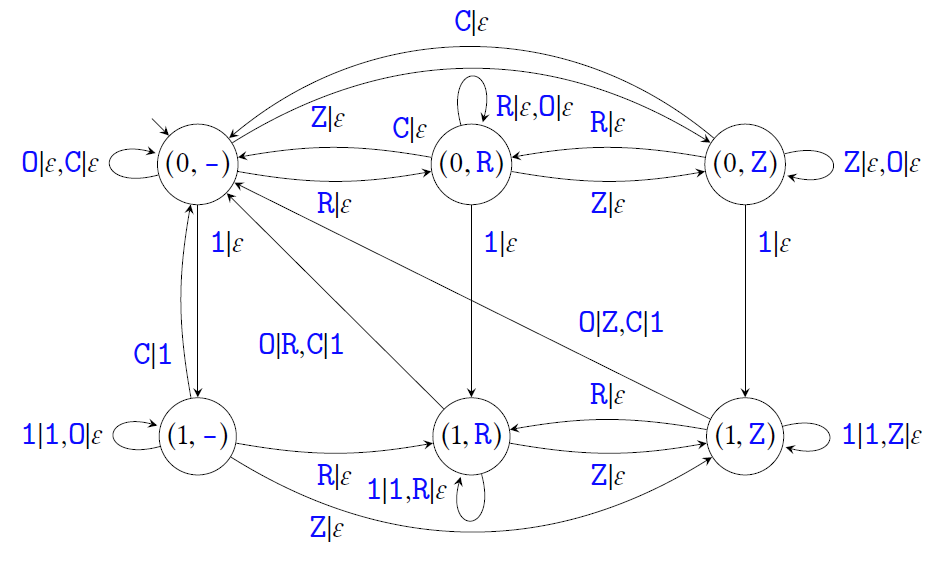
\includegraphics[scale=0.4]{automaten/getraenke} % ist „ohne Ausgabe“ überhaupt erlaubt?? Ich denke nicht.
	\end{figure}
	
	Was ist $f((0,\word -), \word Z), \, f_*((0,\word -), \word{R10}) ,  \, f_{**}( (0,\word -),\word{R10}) $ ? Rechnerisch und graphisch.	
	
\end{frame}

\begin{frame}
	Rechnerisch nur der 3. Fall:
	\begin{threealign}
	f_{**}((0,\word -),\word{R10}) &=& f_{**}((0,\word -),\word{R1}) )\cdot f(f_*((0,\word -),\word{R1}),\word{0}) \\ 
	&=& f_{**} ((0,\word -),\word R) \cdot f(f_*((0,\word -),\word R),\word 1) \\& & \mbox{} \cdot f(f_*((0,\word -),\word{R1}),\word 0) \\ 
	&=& f_{**}((0,\word -),\eps) \cdot f(f_*((0,\word -),\eps),\word R) \\ &&\mbox{} \cdot f(f_*((0,\word -),\word R),\word 1) \cdot f(f_*((0,\word -),\word{R1}),\word 0) \\ 
	&=& (0,\word -) \cdot f((0,\word -),\word R) \cdot f( f(f_*((0,\word -),\eps),\word R),\word 1) \\ &&\mbox{} \cdot f( f(f_*((0,\word -),\word R),\word 1),\word 0) \\
	&=& (0,\word -) \cdot f((0,\word -),\word R) \cdot f( f((0,\word -),\word R),\word 1)  \\& &\mbox{} \cdot f(f(  f(f_*(0,\word -),\eps),\word R),\word 1), \word 0) \\
	&=& (0,\word -) \cdot f((0,\word -),\word R) \cdot f( f((0,\word -),\word R),\word 1)\\ &&\mbox{} \cdot f( f(f((0,\word -),\word R),\word 1),\word 0) \\ 
	&=& (0,\word -) \cdot (0,\word R) \cdot (1,\word R) \cdot (0,\word -) 
	\end{threealign} 
\end{frame}

\begin{frame}{Beispiel}
	\begin{figure}[H]
		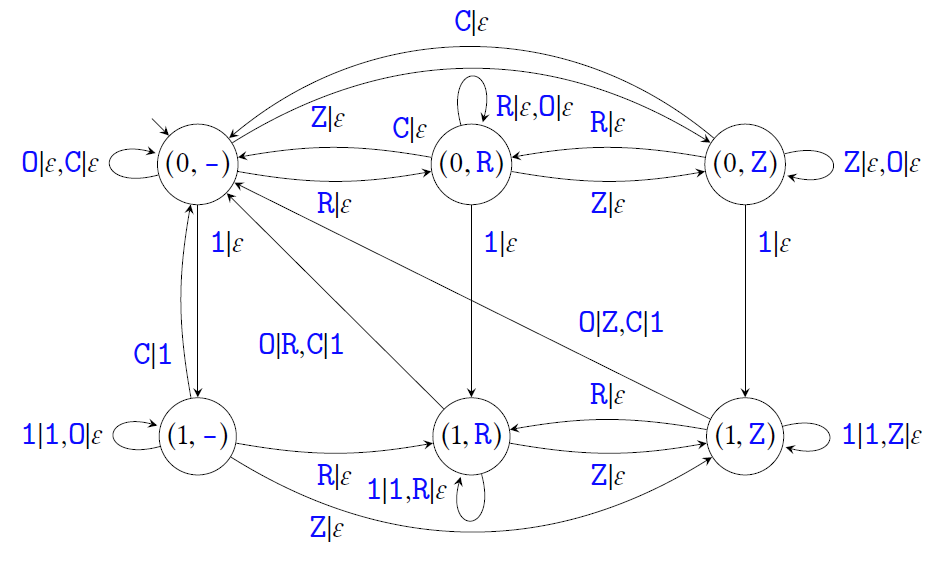
\includegraphics[scale=0.4]{automaten/getraenke}			
	\end{figure}
	Was ist $g_*((0,\word -), \word{R10}) , \, g_{**}((0,\word -),\word{R10}) , \, g_{**}((0,\word -),\word{R110}) $ ? \\ \pause
	$g_*((0,\word -),\word{R10}) = g_{**}((0,\word -),\word{R10}) = \word R, \qquad g_{**}((0,\word -),\word{R110}) = \word{1R} $	
\end{frame}

\begin{frame}{}
	Beispiel: Automaten-Umwandlung (Übung 12, WS 15/16)
\end{frame}

%% Übung: Beispiel
\setbeamercolor{background canvas}{bg=}

\includepdf[pages={34-40}]{U12.pdf}
}